\documentclass[letterpaper]{article}
\usepackage{geometry}
\geometry{margin=1.2in}
\usepackage[protrusion=true,expansion=true]{microtype}  
\usepackage[boxruled,linesnumbered,vlined,inoutnumbered]{algorithm2e}
\usepackage{amsmath}
\usepackage{amsthm}
\usepackage{amssymb}
\usepackage{mathtools}
\usepackage{mathrsfs}
\usepackage{soul}
\usepackage{natbib}
\usepackage{rotating}
\usepackage{gensymb}
\usepackage{lscape}
\usepackage{array}
\usepackage{makecell}
\renewcommand\theadalign{bc}
\renewcommand\theadfont{\bfseries}
\renewcommand\theadgape{\Gape[4pt]}
\renewcommand\cellgape{\Gape[4pt]}
\usepackage{courier}
\usepackage{lipsum}
\usepackage{graphicx}
\usepackage{subcaption}
\usepackage[space]{grffile}
\usepackage{xcolor}
\definecolor{light-grey}{rgb}{0.9,0.9,0.9}
\definecolor{dark-red}{rgb}{0.4,0.15,0.15}
\definecolor{dark-blue}{rgb}{0,0,0.7}
\usepackage{environ}
\setcounter{tocdepth}{2}
\renewcommand{\contentsname}{Table of Contents}
\usepackage{hyperref}
\hypersetup{
    colorlinks, linkcolor={dark-blue},
    citecolor={dark-blue}, urlcolor={dark-blue}
}

\setlength{\parskip}{1em}
\newcommand{\HIGHLIGHT}[1]{\textcolor{blue}{\textbf{#1}}}
\newcommand{\TODO}[1]{\textcolor{red}{\textbf{#1}}}

\begin{document}
%-----------------
%   Homework 4
%-----------------
\newpage
\begin{center}
    \begin{Large}
    COMPSCI 589 Homework 4 - Spring 2023
    \end{Large}
    \\
    \HIGHLIGHT{Pranav Shekar}
    \\
    \HIGHLIGHT{\today}
\end{center}
\addcontentsline{toc}{subsection}{\textbf{Homework 4}}



\vspace{0.25in}
\section{Instructions}

\begin{itemize}
    \item This homework assignment consists of a programming portion. While you may discuss problems with your peers, you must answer the questions on your own and implement all solutions independently. In your submission, do explicitly list all students with whom you discussed this assignment. 
    \item We strongly recommend that you use \LaTeX~to prepare your submission. The assignment should be submitted on Gradescope as a PDF with marked answers via the Gradescope interface. The source code should be submitted via the Gradescope programming assignment as a .zip file. Include with your source code instructions for how to run your code. 
    \item We strongly encourage you to use Python 3 for your homework code. You may use other languages. In either case, you \textit{must} provide us with clear instructions on how to run your code and reproduce your experiments. 
    \item You may \textit{not} use any machine learning-specific libraries in your code, e.g., TensorFlow, PyTorch, or any machine learning algorithms implemented in scikit-learn. You may use libraries like numpy and matplotlib. If you are not certain whether a specific library is allowed, do ask us.
    \item All submissions will be checked for plagiarism using two independent plagiarism-detection tools. Renaming variable or function names, moving code within a file, etc., are all strategies that \textit{do not} fool the plagiarism-detection tools we use. \textcolor{red}{If you get caught, all penalties mentioned in the syllabus \textit{will} be applied---which may include directly failing the course with a letter grade of ``F''}.
    \item The tex file for this homework (which you can use if you decide to write your solution in \LaTeX), as well as the datasets, can be found \href{https://people.cs.umass.edu/~bsilva/courses/CMPSCI_589/Spring2023/homeworks/hw4.zip}{here}.
    \item The automated system will not accept assignments after 11:55pm on May 6. 
\end{itemize}

\newpage

\vspace{1cm}
\section*{Programming Section (100 Points Total)}

In this homework, you will be implementing the backpropagation algorithm to train a neural network. \textbf{Notice that you may \ul{not} use existing machine learning code for this problem: you must implement the learning algorithm entirely on your own and from scratch.} 

%--------------------------------------------

In this assignment, you will:

\begin{itemize}
\item Implement the backpropagation algorithm to train a neural network. Your implementation should support networks with an adjustable number of layers and neurons. For example, it should support training a neural network with two hidden layers---the first one containing 5 neurons and the second one containing 3 neurons; or a neural network with three hidden layers---each one containing 4 neurons. 
\item Implement the regularization mechanism discussed in class, which will be used, here, to try to mitigate overfitting. 
\item Evaluate your neural network using the \textit{stratified cross-validation} strategy that you implemented as part of a previous homework. We recommend using $k=10$ folds. Out of these, $k-1$ folds will be used to train the neural network. The remaining fold---the one not used during training---will be used to evaluate the neural network's performance. You will then repeat this process, thereby generating (and evaluating) $k$ neural networks. The final performance is the average of the performances computed for each of the folds.
\item Evaluate the performance of your neural network on two datasets as a function of three design decisions: the number of layers of the network; the number of neurons in each of the layers; and the regularization parameter. 
\end{itemize}

Each student is free to decide whether to implement the ``standard'' (non-vectorized) version of backpropagation, or the vectorized version of backpropagation---where all quantities relevant to training (i.e., predicted outputs, the value of the cost function $J$, and gradients) are computed using matrix multiplication operations. We recommend that students solve this assignment by using vectorization techniques. This will significantly improve the time to train your neural network, and it will also result in a relatively more straightforward implementation of the backpropagation algorithm.

We are providing students with files describing (for two simple neural networks) \textit{all} the relevant quantities computed by the backpropagation algorithm, step by step. \textbf{These are intended to help you debug your implementation of the backpropagation algorithm.} These files describe, for example, what is the activation of each neuron when the network is presented with a particular training instance; what is the final output/prediction of the network given a particular training instance; what is the $\delta$ value associated with each neuron, as well as the corresponding gradients of each of the weights of the network. Students \textit{should} use the information contained in these files to ensure that the quantities computed by their implementation of backpropagation match all expected values produced by a correct implementation of this learning algorithm. In case, for example, the gradients computed by a student's implementation do not match the expected/correct ones, the student will be able to quickly identify the first point during the execution of their algorithm where one of the quantities produced by their solution does not match the correct/expected one. This should facilitate debugging.


\section{Deliverables and Experiments}

The main objective of this homework is to study how the performance of a trained neural network is affected by \textit{(i)} the neural network architecture (i.e., by the number of layers and neurons); and \textit{(ii)} by the regularization parameter. 

When implementing your neural network, do not forget to add a \textit{bias} input to each neuron, and to ensure that updates to bias weights are performed correctly if regularization is used. For more information, please see the slides of the corresponding lecture. Also, do not forget to properly normalize the attributes of training and test instances whenever appropriate/necessary. 

You are free to choose between two simple stopping criteria. You may, for instance, \textit{(1)} stop if (after presenting all training instances to the network and updating its weights) the cost function $J$ improves by less than some small user-adjusted constant $\epsilon$; or  \textit{(2)} stop after a constant, pre-defined number $k$ of iterations---where each iteration consists of presenting all instances of the training set to the network, computing gradients, and updating the network's weights. You are free to choose which criterion you would like to use. \textit{In all questions below, do not forget to mention explicitly which criterion you used and what was its corresponding hyper-parameter (i.e., $\epsilon$ or $k$). We encourage you to try different possibilities to identify the setting that produces the best possible performance for your algorithm.}

\underline{After} verifying and ensuring the correctness of your solution (by comparing the outputs produced by your backpropagation implementation with the step-by-step examples we provided; please see Section \ref{correctness_verif}), you will be analyzing two \href{https://people.cs.umass.edu/~bsilva/courses/CMPSCI_589/Spring2023/homeworks/hw4.zip}{datasets}:

\textbf{(1) The Wine Dataset}
The goal, here, is to predict the type of a wine based on its chemical contents. The dataset is composed of 178 instances. Each instance is described by 13 \textit{numerical} attributes, and there are 3 classes.

\textbf{(2) The 1984 United States Congressional Voting Dataset}
The goal, here, is to predict the party (Democrat or Republican) of each U.S. House of Representatives Congressperson. The dataset is composed of 435 instances. Each instance is described by 16 \textit{categorical} attributes, and there are 2 classes.

\subsection{Correctness Verification}
\label{correctness_verif}

You will first have to verify that your implementation of backpropagation is correct; that is, that the gradients it computes are accurate. To do this, we are providing each student with two files: \emph{backprop\_example1.txt} and \emph{backprop\_example2.txt}. Each of these files describes a particular neural network architecture and one (minimal) training set. Each file shows, in detail, all intermediate quantities computed by the backpropagation algorithm, which you will then compare with those produced by your algorithm. These quantities include information such as the activation of each neuron when the network is presented with a given input, the final predicted output produced by the network (and the corresponding expected output), the error/cost function, $J$, of the network, the $\delta$ values of each neuron, and the gradients of all weights. 

You \textit{must} ensure that your implementation of backpropagation is correct. To do so, you should write a function capable of reproducing the quantities described in each of the two benchmark files. This function should produce textual output (e.g., by using simple \textit{print} statements) indicating all relevant quantities computed by your implementation of backpropagation---similarly to how they are presented in the provided benchmark files. In other words, as part of your solution to this assignment, you \textit{must} allow us to call this function (that is, the function that shows that your code can reproduce the outputs presented in \emph{backprop\_example1.txt} and \emph{backprop\_example2.txt}), so that we can verify the correctness of your code. The output itself that you generate does not have to be identical to that shown in the benchmark files, but it should include at least, for each training instance and for both datasets: the activation of each neuron; the final predicted output of the network; the expected output; the cost, $J$, associated with that particular instance; the $\delta$ values of each neuron and the gradients of all weights after the network is presented with that training instance; and the final (regularized) gradients after the backpropagation algorithm is done processing all instances in the training set.

\HIGHLIGHT{You should then \textit{(i)} include in your report instructions describing how we (the instructor, staff, and TA's) should run the function you implemented to demonstrate the correctness of your backpropagation algorithm; i.e., the function that produces all results/quantities described above; and \textit{(ii)} \textit{present} in your report the textual output produced by this function, for both provided benchmark files. This part of the assignment is extremely important, and a non-trivial amount of your final grade will depend on us being able to verify that you implemented the backpropagation training algorithm correctly.} We strongly recommend that you only start working on the next part of this assignment \textit{after} you have verified that your implementation of backpropagation is correct. Otherwise, it may be hard (or impossible) for your neural network to properly learn solutions to the proposed problems. 

The two benchmark files we provide (\emph{backprop\_example1.txt} and \emph{backprop\_example2.txt}) are structured as follows. The first line of each file specifies the regularization parameter, $\lambda$, that should be used. After that, you will find a line describing the network structure---the number of neurons in each layer. Recall that the first layer corresponds to the network's input layer and that the last layer corresponds to the output layer. In the notation we adopted here, the bias neuron is \textit{not} included in the neuron counts shown in this line. As an example, consider a neural network with two inputs, one hidden layer with 3 neurons, and one output. In this case, the second line of the provided files would define the network's structure as being [2 3 1]. Notice, however, that (as always) your implementation \textit{should} include bias neurons/weights. We do not typically count them when defining/specifying the architecture of a network because it is implicit that they are always being used. After this section of the file, you will encounter a description of the initial/current weights of the network. Here, each row represents the weights of a given neuron in one particular layer; the weights of the $i$-th neuron are stored in the $i$-th row of the corresponding table/matrix. Recall that the first weight of each neuron corresponds to the bias weight connected to that neuron. Consider the following simple neural network as an example:

    \begin{figure}[!h]
        \centering
        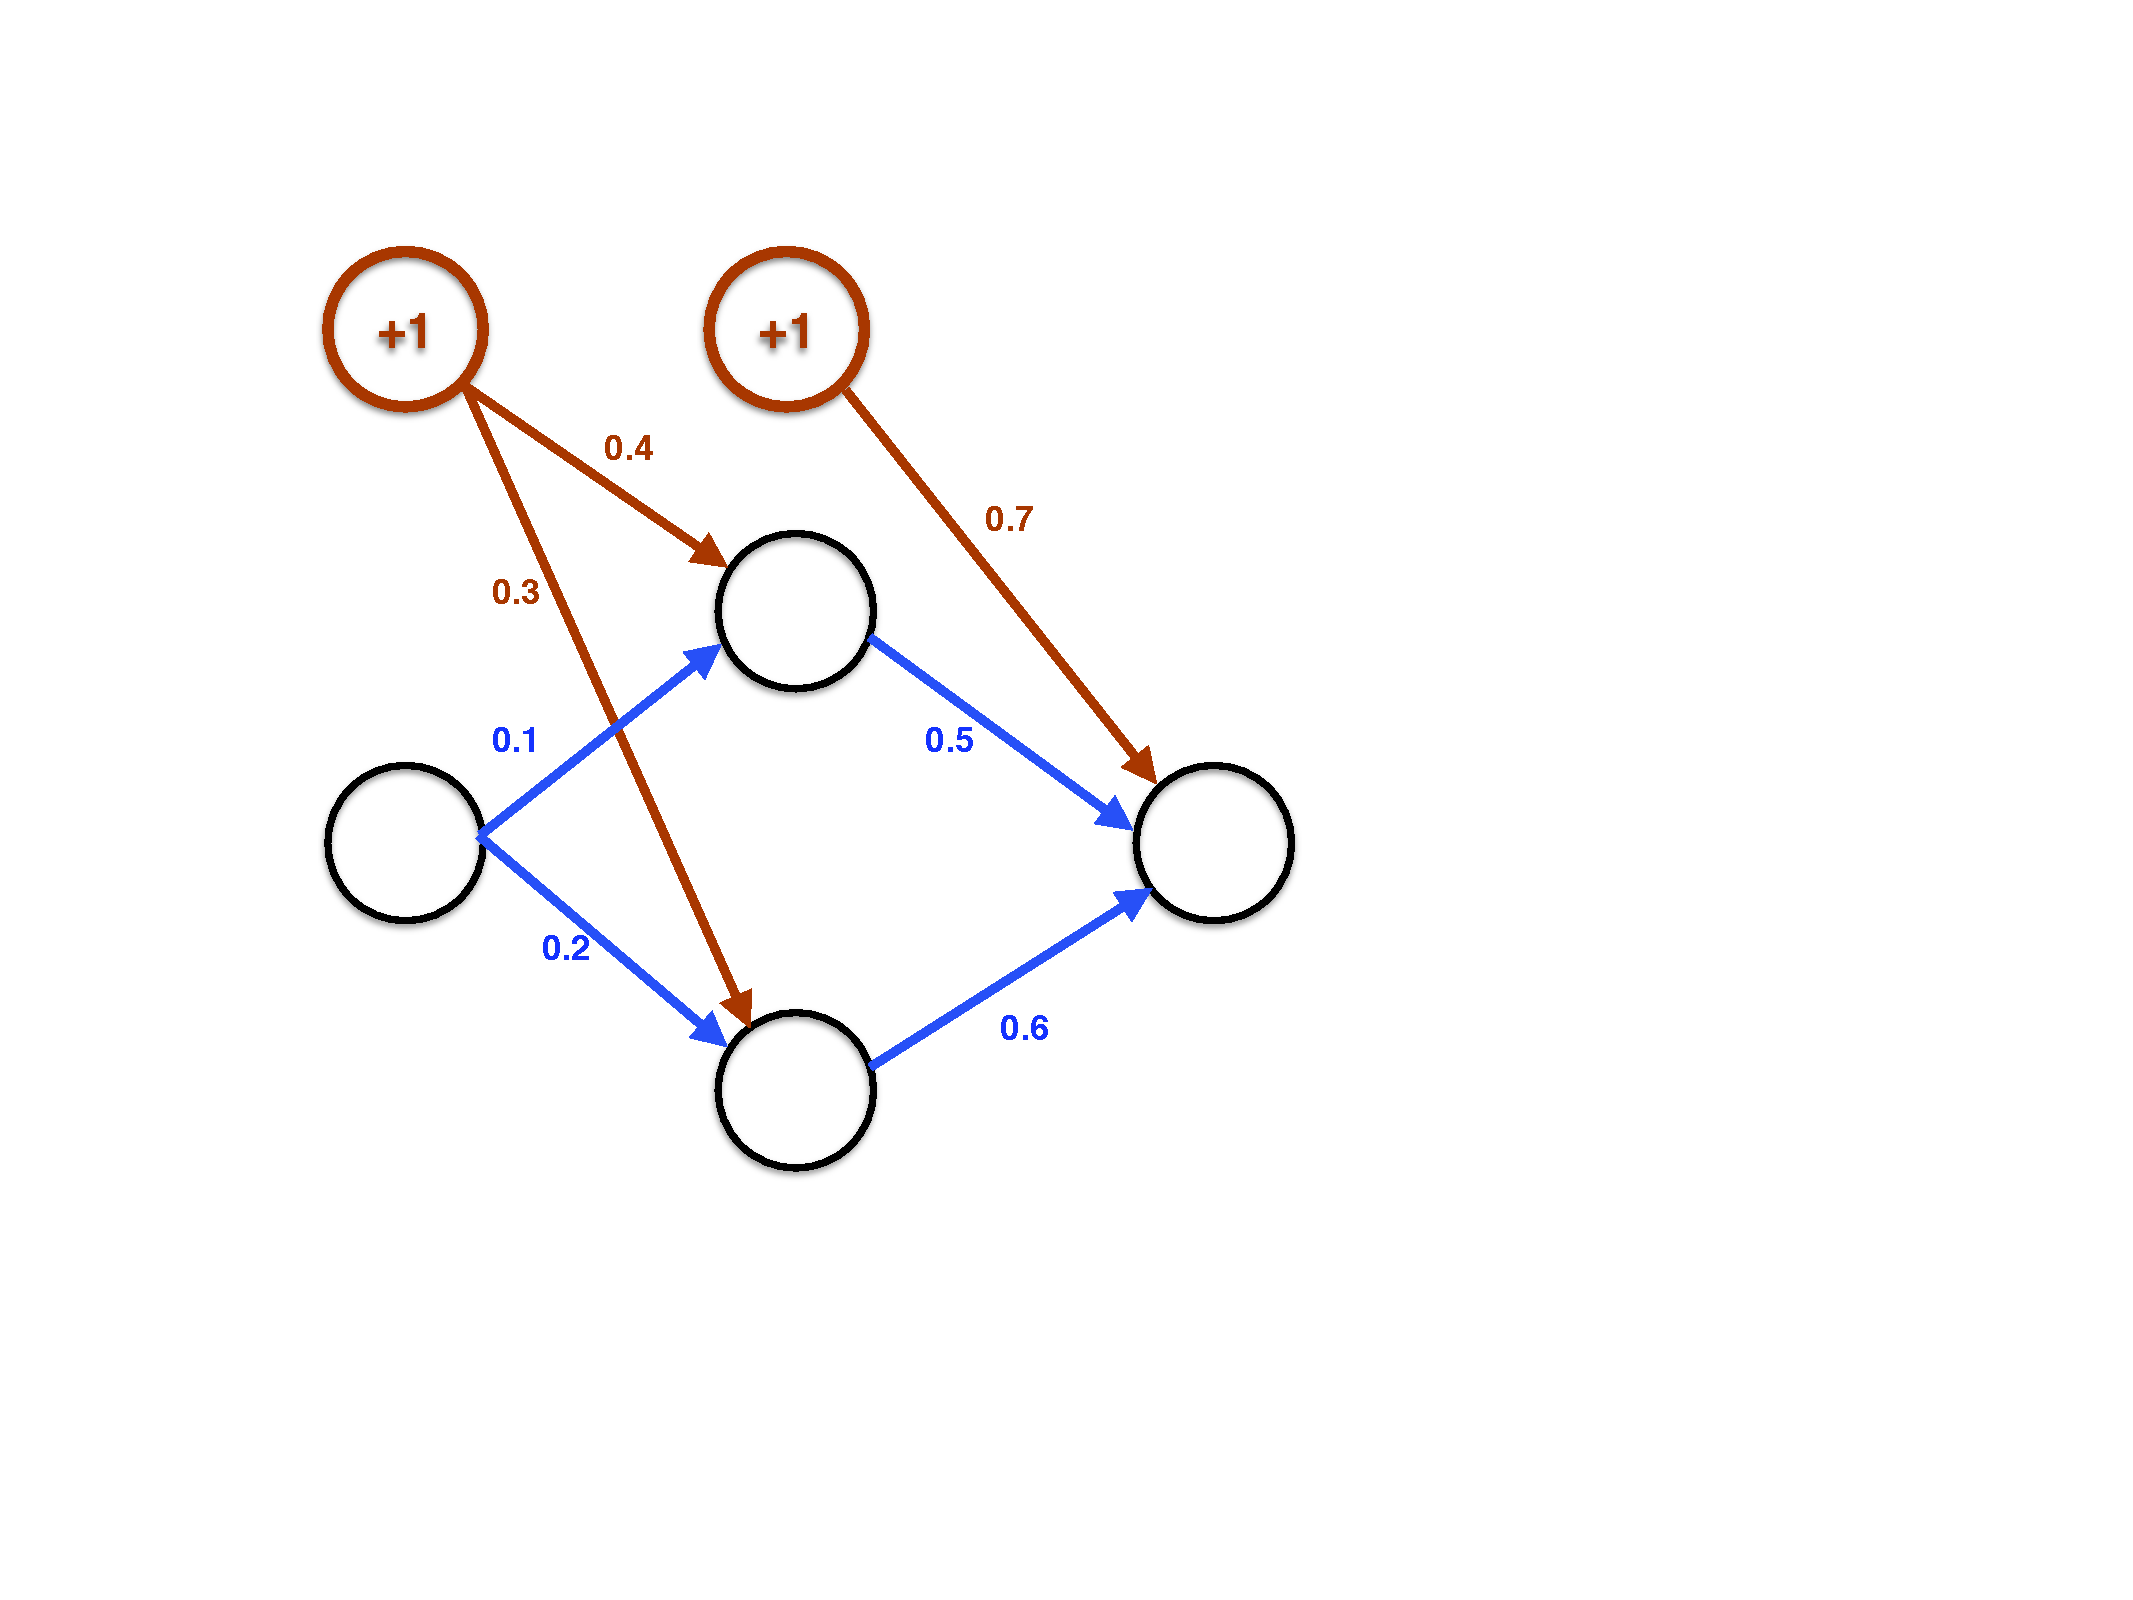
\includegraphics[width=0.3\columnwidth]{figures/network_example.pdf}
    \end{figure}

    \noindent The weights $\theta^{l=1}$ (Theta1) would be shown as follows:
    %
    \begin{verbatim}
     0.4 0.1
     0.3 0.2
    \end{verbatim}
    %
    The weights $\theta^{l=2}$ (Theta2) would be shown as follows:  
    %
    \begin{verbatim}
     0.7 0.5 0.6
    \end{verbatim}

    After this section of the file, you will find a description of the inputs ($x$) and expected outputs ($y$) of each instance in a training set. The subsequent parts of the file show the intermediate quantities computed by the forward propagation process when performed on each of the training instances. In particular, this part of the file shows the $z$ and $a$ values of each neuron (i.e., their activations), as well as the network's final prediction, $f(x)$, and the cost function, $J$, associated with that particular instance. 
    %
    The final section of each presents all intermediate quantities computed by the algorithm during the backpropagation phase: the $\delta$ values of each neuron, after processing a particular training instance, and the gradients of all weights after processing that instance. After that, you will find the final (regularized) gradients of all weights, computed based on all training instances. As discussed in class, these gradients correspond to the gradients based on which we should update the network's weights so that it (on average) makes better predictions for all training examples in the dataset.

\subsection{Experiments and Analyses}

\HIGHLIGHT{For each dataset, you should}:

\begin{enumerate}
    \item Train a neural network and evaluate it using the stratified cross-validation technique discussed in class. You should train neural networks using different values for the regularization parameter, $\lambda$, and using different architectures. You can decide which architectures you will evaluate. As an example, consider testing networks with 1, 2, 3, and 4 hidden layers, and with various numbers of neurons per layer: e.g., 2, 4, 8, 16.
    \item For each trained neural network (i.e., for each combination of architecture and regularization that you tested), you should measure the resulting model's accuracy and F1 score. 
    \item Based on these experiments, you should create, for each dataset and for each of the metrics described above, a table summarizing the corresponding results (i.e., you should show the value of each performance metric for each type of neural network that you tested, on both datasets). \textbf{You should test \textit{at least} 6 neural network architectures on each dataset}. \\ \\
    
    
\HIGHLIGHT{As described in the assignment, I used stratified cross-validation to train and evaluate the neural network with 10 folds. I then varied the regularization parameter and used a couple of different architectures to get the information necessary. The following is a table of the results of tests with six different architectures for the congressional house votes data:} \\

\begin{tabular}{|c|c|c|c|c|c|}
\hline
\# hidden layers & neurons per layer & regularization & accuracy & F1 \\
\hline
1 & 2 & 0 & 0.942016317 & 0.953241031 \\
\hline
2 & 4 & 0.25 & 0.9494172494 & 0.9605262438 \\
\hline
2 & 8 & 0 & 0.9673076923 & 0.9734459316 \\
\hline
3 & 8 & 0.25 & 0.9604895105 & 0.9676671313 \\
\hline
3 & 16 & 0 & 0.9744172494 & 0.979330492 \\
\hline
4 & 16 & 0.25 & 0.9559440559 & 0.9650607226 \\
\hline
\end{tabular} \\ \\


\HIGHLIGHT{The following is a table of the results of tests with six different architectures for the wine data:}

\begin{tabular}{|c|c|c|c|c|}
\hline
\# hidden layers & neurons per layer & regularization & accuracy & F1 \\
\hline
1 & 2 & 0 & 0.9755555556 & 0.9773730578 \\
\hline
2 & 4 & 0.25 & 0.9755555556 & 0.9769738115 \\
\hline
2 & 8 & 0 & 0.9866666667 & 0.9868969435 \\
\hline
3 & 8 & 0.25 & 0.9755555556 & 0.9769738115 \\
\hline
3 & 16 & 0 & 0.9811111111 & 0.9817357663 \\
\hline
4 & 16 & 0.25 & 0.9644444444 & 0.9680486829 \\
\hline
\end{tabular} \\ \\
    
    
    
    \item Discuss (on a high level) what contributed the most to improving performance: changing the regularization parameter; adding more layers; having deeper networks with many layers but few neurons per layer? designing networks with few layers but many neurons per layer? Discuss any patterns that you may have encountered. Also, discuss whether there is a point where constructing and training more ``sophisticated''/complex networks---i.e., larger networks---no longer improves performance (or worsens performance). \\
    
\HIGHLIGHT{The stopping criterion I decided to use was to stop after a predefined $k$ iterations. I chose $k=500$ iterations as I tested a few different numbers and thought that it would be the best number of iterations to do. Trying 250 iterations seemed to still have a bit too much variability in the resulting accuracy and F1 scores. Trying 1000 iterations seemed to always result in about the same accuracy and F1, so in between was the best result.} \\

\HIGHLIGHT{In general, I believe that a mix of the right number of layers and neurons per layer was the best architecture for the neural network. Increasing the number of layers generally helped the accuracy and F1 scores of the data being tested. However, too many layers ended with a resulting loss in both accuracy and F1. The same thing was true for the number of neurons per layer. I found that the best results was usually with 2-3 layers and 8 neurons per layer.} \\

\HIGHLIGHT{Testing different regularization parameters did not seem to change the data much or at all. I believe this is because the number of attributes in the data set. If there were a lot more attributes then the regularization parameter would have had a much greater impact.} \\

\HIGHLIGHT{There is a point where training more "sophisticated" or complex networks would no longer improve performance. If we over complicate the neural network, it can very easily begin overfitting for a specific training set, leading to questionable results on the testing set. This can inevitably lead to stagnant or even worse performance compared to networks that are much simpler in architecture.} \\

    
    \item Based on the analyses above,  discuss which neural network architecture you would select if you had to deploy such a classifier in real life. Explain your reasoning. \\ \\
    
    
\HIGHLIGHT{The neural network architecture I would choose to deploy a real life classifier would be one with 3 layers and 8 neurons per layer. The reason I would choose this architecture is because it most consistently gave me the best results when I was testing. I feel as though a fewer number of layers would be too few and would hinder performance since the neural net wouldn't be "learning" as much, and similarly too many layers would hinder performance since the neural network would be "learning" too much, resulting in overfitting and underfitting. Following the same vein, I believe that 8 neurons per hidden layer is ideal for our test cases since we don't have too many attributes that we are working with. Having too few or too many neurons would lead to a similar scenario that would leave us with potentially bad results compared to a more ideal architecture.} \\
   
    
    \item After identifying the best neural network architecture for each one of the datasets, train it once again on the corresponding dataset and create a learning curve where the $y$ axis shows the network's performance ($J$) on a test set, and where the $x$ axis indicates the number of training samples given to the network. This graph intuitively represents something like this: after showing 5 training examples to the network, what is its performance $J$ on the test set? After showing 10 training examples to the network, what is its performance $J$ on the test set? If the network's parameters and architecture are well-adjusted, this graph should indicate that the network's performance improves as the number of training examples grows; in particular, that $J$ \textit{decreases} as a function of the number of training instances presented to the network. Please also report the step size value, $\alpha$, you used when training this network. \\
    
    
\HIGHLIGHT{The architecture I trained the data on was with 3 hidden layers and 8 neurons per layer. The trend I noticed as the number of instances increased was that the regularized cost decreased, approaching close to 0 and evening out towards the end of each of the data sets. When doing these calculations, I set the regularization to 0 and the step size to 1 as I got the most consistent results with those values.}   \\

\HIGHLIGHT{The following table is the trend of the cost function for the house votes data:} \\

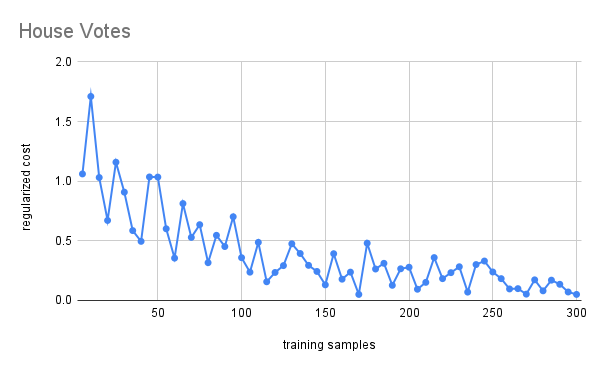
\includegraphics[scale=.75]{House Votes.png} \\

\HIGHLIGHT{The following table is the trend of the cost function for the wine data:} \\

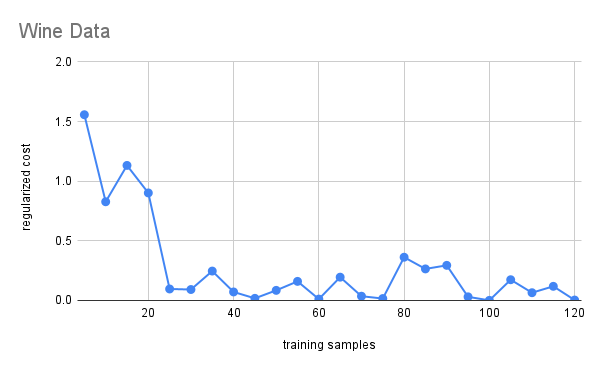
\includegraphics[scale=.75]{Wine Data.png} \\
    

    \item Although this last step/task is not required, we recommend that you train the network using the mini-batch gradient descent approach. You can manually select and adjust the mini-batch size that you would like to use. Training a neural network in this way significantly accelerates the training process.
    
\end{enumerate}

\section{Some Hints}

\begin{enumerate}
    \item Initialize the network's weights with small random numbers from -1 to +1 or random numbers sampled from a Gaussian distribution with zero mean and variance equal to 1.
    \item When trying to identify effective network architectures, start your investigation by testing networks with few layers (e.g., try, first, networks with just one hidden layer). Increase the number of layers---and/or the number of neurons per layer---only when necessary.
    \item When training a given neural network architecture, try, first, to use larger step sizes, $\alpha$. If you set $\alpha$ too small, the training process may become very slow or prematurely converge to a bad local minimum (depending on the stopping criterion you use). By contrast, if the network's performance oscillates significantly during training when using large values of $\alpha$, you might be overshooting. In this case, decrease the value of $\alpha$. Repeat this process until you find the largest step size that can be effectively used---i.e., the value that allows the weights to be updated fairly quickly, but that does not cause weight instability or divergence.
    \item After you identify a value of $\alpha$ that causes the network's performance to improve in a reasonably consistent way, check the performance (value of $J$) to which the network converges. If it is not satisfactory, your network architecture might be too simple (i.e., the network might be underfitting). In this case, try to increase the number of layers and/or the number of neurons per layer. Then, repeat the analyses above regarding how to evaluate different step sizes, $\alpha$.

\end{enumerate}


\vspace{1cm}
\noindent\rule{\textwidth}{1pt}

\textbf{There are four ways in which we may receive extra credit in this homework.}

\noindent \HIGHLIGHT{(Extra Points \#1: 13 Points)} 
Implement the vectorized form of backpropagation. As previously mentioned, this is not mandatory, but you can get extra credit if you do it. Most modern implementations of neural networks use vectorization, so it is useful for you to familiarize yourself with this type of approach. \\

\HIGHLIGHT{The backpropagation that I implemented uses the vectorized form.} \\


\noindent \HIGHLIGHT{(Extra Points \#2: 13 Points)} 
Analyze a third dataset: the \textbf{Breast Cancer Dataset}. The goal, here, is to classify whether tissue removed via a biopsy indicates whether a person may or may not have breast cancer. There are 699 instances in this dataset. Each instance is described by 9 \textit{numerical} attributes, and there are 2 classes. You should present the same analyses and graphs as discussed above. This dataset can be found in the same zip file as the two main datasets. \\

\HIGHLIGHT{The table for the cancer data is presented below:}

\begin{tabular}{|c|c|c|c|c|}
\hline
\# hidden layers & neurons per layer & regularization & accuracy & F1 \\
\hline
1 & 2 & 0 & 0.9684453782 & 0.9755773195 \\
\hline
2 & 4 & 0.25 & 0.9627310924 & 0.9712480878 \\
\hline
2 & 8 & 0 & 0.9641596639 & 0.9723526295 \\
\hline
3 & 8 & 0.25 & 0.9641596639 & 0.9723973625 \\
\hline
3 & 16 & 0 & 0.9627310924 & 0.9717680641 \\
\hline
4 & 16 & 0.25 & 0.9669747899 & 0.9746223514 \\
\hline
\end{tabular} \\

\HIGHLIGHT{Similar to the other two data sets, the stopping criterion I used was a predefined 500 iterations. Also, similar to the other data sets, The best results were found with 2-3 layers and 8 neurons per layer. The regularization parameter again didn't seem to have much of an impact on the results of the tests I ran, again probably due to the small number of attributes we are testing with.} \\

\HIGHLIGHT{The architecture I chose as the best for this neural net is again 3 layers with 8 neurons per layer. The trend was similar again to the previous two data sets, with the regularized cost decreasing as the number of instances increased. Similarly, I set the regularization parameter to 0 and the step size to 1 as I got the best results with those values. The graph of the resulting cost data is below:} \\

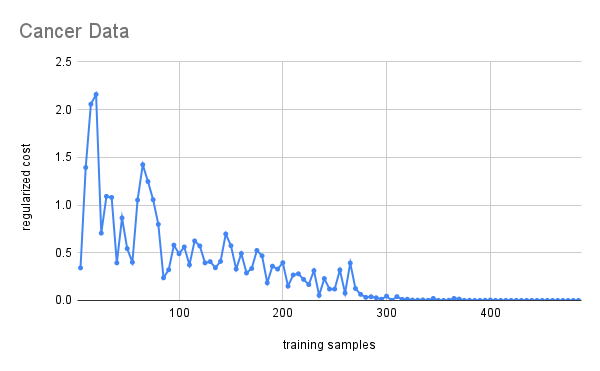
\includegraphics[scale=.75]{Cancer Data.png} \\

\HIGHLIGHT{After around 300 instances, the regularized cost seems to even out very close to 0 and stay low for any increase in training samples.} \\



\noindent \HIGHLIGHT{(Extra Points \#3: 13 Points)}    
Analyze a fourth, more challenging dataset: the \textbf{Contraceptive Method Choice Dataset}. The goal, here, is to predict the type of contraceptive method used by a person based on many attributes describing that person. This dataset is more challenging because it combines \textit{both numerical and categorical attributes}. There are 1473 instances in this dataset. Each instance is described by 9 attributes, and there are 3 classes. The dataset can be downloaded \href{https://archive.ics.uci.edu/ml/datasets/Contraceptive+Method+Choice}{here}. You should present the same analyses and graphs discussed above.

\noindent \HIGHLIGHT{(Extra Points \#4: 13 Points)}
Implement the method (discussed in class) that allows you to \textit{numerically} check the gradients computed by backpropagation. This will allow you to further ensure that all gradients computed by your implementation of backpropagation are correct; that way, you will be confident that you trust your implementation of the neural network training procedure. You should present in your report the estimated gradients for the two neural networks described on the provided benchmark files. First, estimate the gradients using $\epsilon=0.1$, and then $\epsilon=0.000001$. If you choose to work on this extra-credit task, please include the corresponding source code along with your Gradescope submission.


\end{document}

